% Template for PLoS
% Version 3.4 January 2017
%
% % % % % % % % % % % % % % % % % % % % % %
%
% -- IMPORTANT NOTE
%
% This template contains comments intended 
% to minimize problems and delays during our production 
% process. Please follow the template instructions
% whenever possible.
%
% % % % % % % % % % % % % % % % % % % % % % % 
%
% Once your paper is accepted for publication, 
% PLEASE REMOVE ALL TRACKED CHANGES in this file 
% and leave only the final text of your manuscript. 
% PLOS recommends the use of latexdiff to track changes during review, as this will help to maintain a clean tex file.
% Visit https://www.ctan.org/pkg/latexdiff?lang=en for info or contact us at latex@plos.org.
%
%
% There are no restrictions on package use within the LaTeX files except that 
% no packages listed in the template may be deleted.
%
% Please do not include colors or graphics in the text.
%
% The manuscript LaTeX source should be contained within a single file (do not use \input, \externaldocument, or similar commands).
%
% % % % % % % % % % % % % % % % % % % % % % %
%
% -- FIGURES AND TABLES
%
% Please include tables/figure captions directly after the paragraph where they are first cited in the text.
%
% DO NOT INCLUDE GRAPHICS IN YOUR MANUSCRIPT
% - Figures should be uploaded separately from your manuscript file. 
% - Figures generated using LaTeX should be extracted and removed from the PDF before submission. 
% - Figures containing multiple panels/subfigures must be combined into one image file before submission.
% For figure citations, please use "Fig" instead of "Figure".
% See http://journals.plos.org/plosone/s/figures for PLOS figure guidelines.
%
% Tables should be cell-based and may not contain:
% - spacing/line breaks within cells to alter layout or alignment
% - do not nest tabular environments (no tabular environments within tabular environments)
% - no graphics or colored text (cell background color/shading OK)
% See http://journals.plos.org/plosone/s/tables for table guidelines.
%
% For tables that exceed the width of the text column, use the adjustwidth environment as illustrated in the example table in text below.
%
% % % % % % % % % % % % % % % % % % % % % % % %
%
% -- EQUATIONS, MATH SYMBOLS, SUBSCRIPTS, AND SUPERSCRIPTS
%
% IMPORTANT
% Below are a few tips to help format your equations and other special characters according to our specifications. For more tips to help reduce the possibility of formatting errors during conversion, please see our LaTeX guidelines at http://journals.plos.org/plosone/s/latex
%
% For inline equations, please be sure to include all portions of an equation in the math environment.  For example, x$^2$ is incorrect; this should be formatted as $x^2$ (or $\mathrm{x}^2$ if the romanized font is desired).
%
% Do not include text that is not math in the math environment. For example, CO2 should be written as CO\textsubscript{2} instead of CO$_2$.
%
% Please add line breaks to long display equations when possible in order to fit size of the column. 
%
% For inline equations, please do not include punctuation (commas, etc) within the math environment unless this is part of the equation.
%
% When adding superscript or subscripts outside of brackets/braces, please group using {}.  For example, change "[U(D,E,\gamma)]^2" to "{[U(D,E,\gamma)]}^2". 
%
% Do not use \cal for caligraphic font.  Instead, use \mathcal{}
%
% % % % % % % % % % % % % % % % % % % % % % % % 
%
% Please contact latex@plos.org with any questions.
%
% % % % % % % % % % % % % % % % % % % % % % % %

\documentclass[10pt,letterpaper]{article}
\usepackage[top=0.85in,left=2.75in,footskip=0.75in]{geometry}

% amsmath and amssymb packages, useful for mathematical formulas and symbols
\usepackage{amsmath,amssymb}

% Use adjustwidth environment to exceed column width (see example table in text)
\usepackage{changepage}

% Use Unicode characters when possible
\usepackage[utf8x]{inputenc}

% textcomp package and marvosym package for additional characters
\usepackage{textcomp,marvosym}

% cite package, to clean up citations in the main text. Do not remove.
\usepackage{cite}

% Use nameref to cite supporting information files (see Supporting Information section for more info)
\usepackage{nameref,hyperref}

% line numbers
\usepackage[right]{lineno}

% ligatures disabled
\usepackage{microtype}
\DisableLigatures[f]{encoding = *, family = * }

% color can be used to apply background shading to table cells only
\usepackage[table]{xcolor}

% array package and thick rules for tables
\usepackage{array}

% NOT part of PLOS TEMPLATE, remove before sending?
\usepackage{todonotes}
\usepackage{wrapfig}
\usepackage{url}

% create "+" rule type for thick vertical lines
\newcolumntype{+}{!{\vrule width 2pt}}

% create \thickcline for thick horizontal lines of variable length
\newlength\savedwidth
\newcommand\thickcline[1]{%
	\noalign{\global\savedwidth\arrayrulewidth\global\arrayrulewidth 2pt}%
	\cline{#1}%
	\noalign{\vskip\arrayrulewidth}%
	\noalign{\global\arrayrulewidth\savedwidth}%
}

% \thickhline command for thick horizontal lines that span the table
\newcommand\thickhline{\noalign{\global\savedwidth\arrayrulewidth\global\arrayrulewidth 2pt}%
	\hline
	\noalign{\global\arrayrulewidth\savedwidth}}


% Remove comment for double spacing
%\usepackage{setspace} 
%\doublespacing

% Text layout
\raggedright
\setlength{\parindent}{0.5cm}
\textwidth 5.25in 
\textheight 8.75in

% Bold the 'Figure #' in the caption and separate it from the title/caption with a period
% Captions will be left justified
\usepackage[aboveskip=1pt,labelfont=bf,labelsep=period,justification=raggedright,singlelinecheck=off]{caption}
\renewcommand{\figurename}{Fig}


% Remove brackets from numbering in List of References
\makeatletter
\renewcommand{\@biblabel}[1]{\quad#1.}
\makeatother

% Leave date blank
\date{}

% Header and Footer with logo
\usepackage{lastpage,fancyhdr,graphicx}
\usepackage{epstopdf}
\pagestyle{myheadings}
\pagestyle{fancy}
\fancyhf{}
\setlength{\headheight}{27.023pt}
\lhead{
\includegraphics[width=2.0in]{PLOS-submission.eps}}
\rfoot{\thepage/\pageref{LastPage}}
\renewcommand{\footrule}{\hrule height 2pt \vspace{2mm}}
\fancyheadoffset[L]{2.25in}
\fancyfootoffset[L]{2.25in}
\lfoot{\sf PLOS}

%% Include all macros below

\newcommand{\lorem}{{\bf LOREM}}
\newcommand{\ipsum}{{\bf IPSUM}}

%% END MACROS SECTION


\begin{document}
	\vspace*{0.2in}
	
	% Title must be 250 characters or less.
	\begin{flushleft}
		{\Large
			\textbf\newline{TFEA.ChIP: A tool kit for transcription factor binding site enrichment analysis capitalizing on ChIP-seq datasets} % Please use "sentence case" for title and headings (capitalize only the first word in a title (or heading), the first word in a subtitle (or subheading), and any proper nouns).
		}
		\newline
		% Insert author names, affiliations and corresponding author email (do not include titles, positions, or degrees).
		\\
		Laura Puente-Santamaria\textsuperscript{1},
		Luis del Peso\textsuperscript{1,2,3*}
		\\
		\bigskip
		\textbf{1} Departamento de Bioquímica, Universidad Autónoma de Madrid (UAM) and Instituto de Investigaciones Biomédicas 'Alberto Sols' (CSIC-UAM), 28029 Madrid , Spain
		\\
		\textbf{2} IdiPaz, Instituto de Investigación Sanitaria del Hospital Universitario La Paz, 28029 Madrid, Spain.
		\\
		\textbf{3} CIBER de Enfermedades Respiratorias (CIBERES), Instituto de Salud Carlos III, 28029 Madrid, Spain.
		\\
		\bigskip
		
		% Insert additional author notes using the symbols described below. Insert symbol callouts after author names as necessary.
		% 
		% Remove or comment out the author notes below if they aren't used.
		%
		% Primary Equal Contribution Note
		%\Yinyang These authors contributed equally to this work.
		
		% Additional Equal Contribution Note
		% Also use this double-dagger symbol for special authorship notes, such as senior authorship.
		%\ddag These authors also contributed equally to this work.
		
		% Current address notes
		%\textcurrency Current Address: Dept/Program/Center, Institution Name, City, State, Country % change symbol to "\textcurrency a" if more than one current address note
		% \textcurrency b Insert second current address 
		% \textcurrency c Insert third current address
		
		% Deceased author note
		%\dag Deceased
		
		% Group/Consortium Author Note
		%\textpilcrow Membership list can be found in the Acknowledgments section.
		
		% Use the asterisk to denote corresponding authorship and provide email address in note below.
		* luis.peso@uam.es
		
	\end{flushleft}
	% Please keep the abstract below 300 words
	\section*{Abstract}
	The identification of transcription factor (TF) responsible for the co-regulation of an specific set of genes is a common problem in transcriptomics. With the development of TFEA.ChIP we aim to provide a tool to estimate and visualize TF enrichment in a set of differentially expressed genes that takes into account the wide variation in TF's behavior across different cell types and stimuli. To that end, ChIP-Seq experiments from the ENCODE Consortium and GEO Datasets were gathered, and a database linking TFs with the genes they interact with in each ChIP-Seq experiment was generated. In its current state, TFEA.ChIP covers 333 different transcription factors from 1122 ChIP-Seq experiments, with over 150 cell types being represented. The analysis of publicly available RNAseq datasets, including hypoxic transcriptomes and response to cytokines, show that TFEA.ChIP accurately identifies the relevant transcription factors in each case. The use of ChIP-Seq data instead of PWM-based methods allows to expand the analysis of TF enrichment to include cofactors that lack a DNA binding domain as well as chromatin modifiers, in addition to provide a biological context to infer tissue and stimuli-dependent TF behavior. TFEA.ChIP is available as a Bioconductor package at: \url{https://www.bioconductor.org/packages/devel/bioc/html/TFEA.ChIP.html} 
	\todo[size=\tiny, backgroundcolor= yellow!50 ]{Include here comparison with Opossum and results.}
	
	
	% Please keep the Author Summary between 150 and 200 words
	% Use first person. PLOS ONE authors please skip this step. 
	% Author Summary not valid for PLOS ONE submissions.   
	\section*{Author summary}
	[I believe this is required for research articles, but not software papers.]
	\todo[size=\tiny, backgroundcolor= yellow!50 ]{Methods articles and Software articles require presubmission inquiries.} 
	\linenumbers
	
	% Use "Eq" instead of "Equation" for equation citations.
	\section*{Introduction}
	In the most simple scenario, the comparison of the transcriptome of cells or organisms in two conditions leads to the identification of a set of differentially expressed (DE) genes, and the underlying assumption is that one or a few TFs regulate the expression of those genes. Traditionally, the identification of relevant TFs has relied on the use of position weight matrices (PWMs) to predict transcription factor binding sites (TFBSs) proximal to the DE genes\cite{Wasserman}. The comparison of predicted TFBS in DE versus a set of control genes, reveals factors that are significantly enriched in the DE gene set. The prediction of TFBS using these approaches have been useful to narrow down potential binding sites, but can suffer from high rates of false positives. In addition, this approach is limited by design to sequence-specific transcription factors (TF) and thus unable to identify cofactors that bind indirectly to target genes. To overcome these limitations we developed the R package TFEA.ChIP, which exploits the vast amount of publicly available ChIP-Seq datasets to determine TFBS proximal to a given set of genes and computes enrichment analysis based on this experimentally-derived rich information. Specifically TFEA.ChIP, uses information derived from the hundreds of ChIP-Seq experiments from the ENCODE Consortium\cite{ENCODE} expanded to include additional datasets contributed to GEO database\cite{GEO1}\cite{GEO2} by individual laboratories representing the binding sites of factors not assayed by ENCODE. The package includes a set of tools to customize the ChIP data, perform enrichment analysis and visualize the results. Herein we describe the main characteristics of the package and compare the results produced by TFEA.ChIP vs those generated by Oppossum, an state of the art TFBS identification software based on PWMs \cite{Kwon2012}. Our data indicate that the results of TFEA.ChIP and Opossum are coincident for those datasets where Oppossum identifies clear TFBS candidate(s). In addition, TFEA.ChIP identified enriched factors for some data sets where Opossum was unable to find a significant match.\todo[size=\tiny, backgroundcolor= yellow!50]{Indicate that the factors found by TFEA.ChP are the ones expected according to the experimental manipulations in each dataset.}
	
	\section*{Design and implementation}
	\subsection*{Database}
	TFEA.ChIP package includes analysis and visualization tools intended for the identification of TFBS enriched in a set of DE genes. To this end, the package uses experimental information derived from 1122 ChIP-seq datasets, generated by the ENCODE consortium and individual researchers, testing a total of 333 individual human transcription factors in a variety of cell types and experimental conditions. The collection of TF includes both sequence-specific transcription factors as well as molecules that bind DNA indirectly (e.g. transcription cofactors and chromatin modifiers) or in a sequence-independent fashion (e.g. RNA Polymerases). This is an important difference with methods based on PWMs that, by design, are restricted to sequence-specific factors. The database includes a total of XX of sequence-specific TF (XX\% of total factors). Thus, this compiled database covers XX-XX\% of the 1,391\cite{TFcensus} to ~1600 \cite{Lambert2018} transcription factors estimated to be encoded by the human genome. In addition, the set includes proteins from all the major classes of DNA binding domains (Fig~\ref{fig1}).
	\todo[size=\tiny, backgroundcolor= yellow!50 ]{Indicate number and percentage of seq-specific TF above}
	
	% Place figure captions after the first paragraph in which they are cited.
	\todo[size=\tiny, backgroundcolor= yellow!50 ]{remove before submission. Figures must be send separately}	
	\todo[size=\tiny, backgroundcolor= yellow!50 ]{this is just an example taken from ref. Vaquerizas et al. Indicate How the classification was done. Also, if possible, adhere to the classification indicated in Vaquerizas et al or Lambert et al}
	%\begin{wrapfigure}{r}{0.55\textwidth}
	
	\begin{figure}[!h]
		\centering
		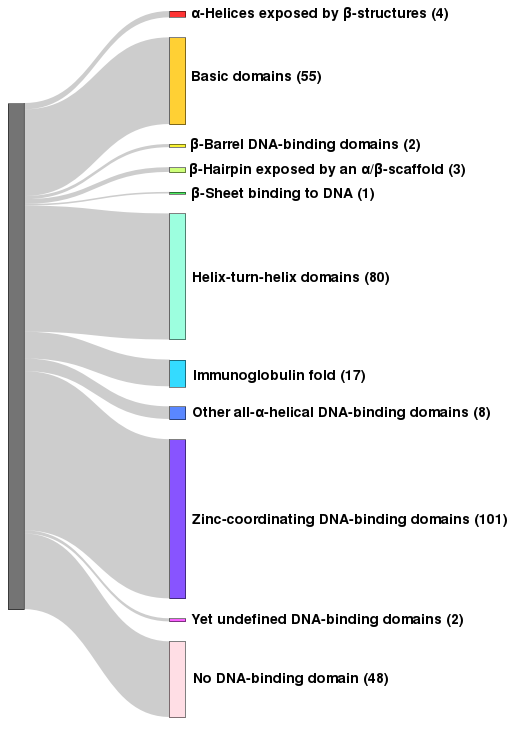
\includegraphics[width=0.5\textwidth]{superclases}
		\caption{{\bf Structural diversity according to DNA-binding domains of the transcription factors included in the TFBS database.} The 333 TFs included in TFEA.ChIP database were classified into families according to their DNA-binding domain composition. InterPro parent–child relationships between DNA-binding domains were used as the basis for TF family definition (Supplementary information S1 (PDF)). TFs with multiple DNA-binding domains were classified in each of their respective families. Families with less than five members were classified as ‘other’.}
		\label{fig1}
	\end{figure} 
	%\end{wrapfigure}
	
	The supplementary table \nameref{S1_Table} contains the complete list of the datasets included in the package along with their GEO accession numbers. \todo[size=\tiny, backgroundcolor= yellow!50 ]{Prepare this table}.  
	\todo[size=\tiny, backgroundcolor= yellow!50 ]{Adding mention to web implementation if done.}
	ChIPseq datasets contain the coordinates of TF binding sites throughout the genome. Thus, in order to use this information in gene enrichment analyses, we first need to associate binding regions (ChIP peaks) to specific genes. In the absence of three-dimensional contact information, such as that produced by Hi-C experiments, the peaks are usually assigned to the nearest gene [REFERENCE NEEDED!]. However, the uncertainty of peak assignation decreases as the distance to the nearest gene increases \cite{Mifsud2015}. For these reasons, we purged the ChIP-seq datasets to remove peaks mapping far from genes. In addition, we also filtered the binding regions to keep only high confidence peaks, as determined by statistical significance (adjusted p-values < 0.05) and overlap with open chromatin regions \cite{EncodeDHS2}. To this end, we first generated a database pairing open chromatin regions, as defined by clusters of Dnase Hypersensitive Sites (DHSs) e\cite{EncodeDHS1}\cite{EncodeDHS2}, and genes in the UCSC Known Gene database (version 3.2.2)\cite{KnownGene}. DHSs were assigned to genes overlapping with the open chromatin region allowing for 1Kb margin from the gene boundaries and multiple gene assignation was allowed for those DHSs overlapping two genes. The final database only retained DHSs that were assigned to at least one gene (Fig~\ref{fig2}, step A). Then, for each ChIP-seq dataset we selected those peaks that were statistically significant and overlaped an open chromatin region in the DHSs-gene database. Each of these peaks was assigned to the same gene as the DHS they overlaped (Fig~\ref{fig2}, step B). Finally, we integrated the peak-gene information from all ChIP-dataset into a binary matrix with rows corresponding to all the human genes in the Known Gene database, and a columns for every ChIP-Seq experiment analyzed; the entry values were assigned to 1 when the row gene had at least one peak assigned in the ChIP-Seq column and 0 otherwise (Fig~\ref{fig2}). It is worth noting that, as a result of the matching strategy, the interaction matrix contains a large fraction of TFBS-gene pairs involving intronic regions which representing distant regulatory interactions \cite{Mifsud2015}.
	
	\begin{figure}[h]
		\centering
		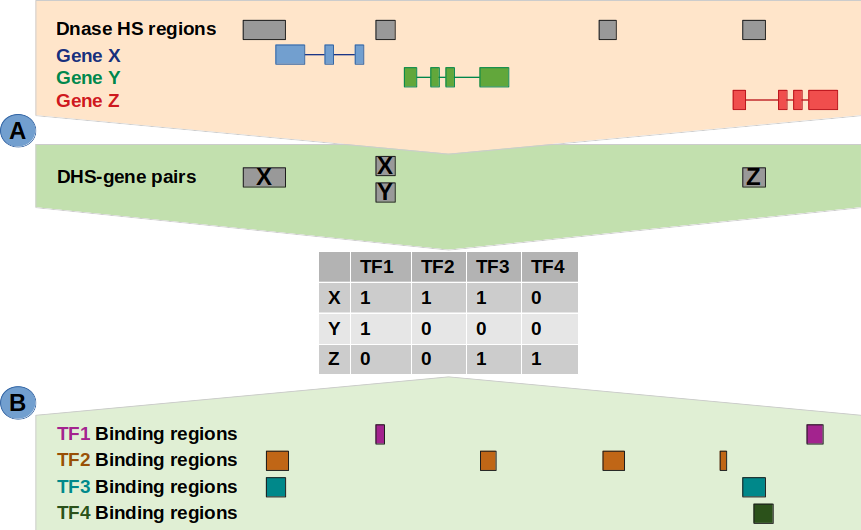
\includegraphics[width=0.8\textwidth]{fig2_LPO}
		\caption{{\bf Building Database of TF-gene associations.} A, We selected open chromatin regions (defined as clusters of DHSs identified by the ENCODE project) that are 1Kb or closer to any of the genes in the UCSC Known Gene database and assign them to the nearest gene(s). B, for every peak in each of the ChIP datasets we selected those overlapping any of the DHSs indicated in A and assigned the peak to the gene represented by the DHSs.}
		\label{fig1}
	\end{figure}
	
	\subsection*{Enrichment analysis}
	TFEA.ChIP is designed to take the output of a differential expression analysis and identify transcription factors enriched in the list of differentially expressed genes. The core premise of our method is that key effectors of a regulatory response will have more target genes among the differentially expressed than among the unresponsive genes. TFEA.ChIP implements to types of tests to identify enriched TF. The first one analyzes the association of TFBS and differential expression from 2x2 tables recording the presence of binding sites for a given TF in DE and control genes. The statistical significance of the association for each transcription factor determined by a Fisher’s exact test. This analysis only requires a list of DE genes as input. In the second method, the association of TF to DE genes is determined using a Gene Set Enrichment Analysis (GSEA)\cite{GSEA1}. This analysis requires a sorted list of genes where gene order reflects the relative expression in each of the two conditions being compared.
	
	\subsection*{Software features}
	\todo[size=\tiny, backgroundcolor= yellow!50 ]{Include Here a brief description of the main functions of the sofware package. See ROTS paper as example.}
	
	% Results and Discussion can be combined.
	\section*{Results}
	The benefits of the use of ChIP-seq data over PWM for the identification of TFBS have been recently shown \cite{Tiana2018a}. The implementation of this approach in the package TFEA.Chip described herein greatly simplifies it application to any general case. Here, we used four case studies to demonstrate the performance of the strategy implemented in this package when applied to different study settings. This cases include the original dataset where a primitive version of this strategy was first tested (transcriptional response of HUVEC cells to hypoxia), two additional datasets where the transcriptional response to the chemokines TNFalpha and IFNalpha was analyzed in different cell lines and a final dataset that, unlike the previous ones, recorded the transcriptional response to a complex pathological situation in vivo rather than to a defined stimulus. In all the cases we compared the output of TFEA.ChIP with the results of oPOSSUM, a PWM-based state-of-the-art tool \cite{Kwon2012}. To compare both methods we took the raw output from oPOSSUM and generated contingency matrices with the number of target hits, target non-hits, background hits, and background non-hits for every PWM, and then performed Fisher’s exact test. The resulting p-values were adjusted for multiple testing using FDR method.
	
	\subsection{Hypoxia vs normoxia in HUVEC cells}
	
	\subsection{TNF addition in neutrophils and adipocytes}
	
	\subsection{Left ventricular non-compaction in cardiomyocytes}
	
	\subsection{INF addition in hESC cells for 15 and 21 days}
	
	\section*{Discussion}
	LIMITATION OF THE CURRENT VERSION: Although the package is mainly focused towards analyzing expression data generated from human cells, TFEA.ChIP includes the option to use datasets derived from experiments in mice, translating mouse gene names to their equivalent ID on the human genome. INDICATE THAT WE ARE ASSUMING THAT TF regulate same genes in different species
	DISCUSS LIMITATION OF 1Kb for association and the possibility of custom-generated DB
	
	\section*{Conclusion}
	
	CO\textsubscript{2} Maecenas convallis mauris sit amet sem ultrices gravida. Etiam eget sapien nibh. Sed ac ipsum eget enim egestas ullamcorper nec euismod ligula. Curabitur fringilla pulvinar lectus consectetur pellentesque. Quisque augue sem, tincidunt sit amet feugiat eget, ullamcorper sed velit. 
	
	Sed non aliquet felis. Lorem ipsum dolor sit amet, consectetur adipiscing elit. Mauris commodo justo ac dui pretium imperdiet. Sed suscipit iaculis mi at feugiat. Ut neque ipsum, luctus id lacus ut, laoreet scelerisque urna. Phasellus venenatis, tortor nec vestibulum mattis, massa tortor interdum felis, nec pellentesque metus tortor nec nisl. Ut ornare mauris tellus, vel dapibus arcu suscipit sed. Nam condimentum sem eget mollis euismod. Nullam dui urna, gravida venenatis dui et, tincidunt sodales ex. Nunc est dui, sodales sed mauris nec, auctor sagittis leo. Aliquam tincidunt, ex in facilisis elementum, libero lectus luctus est, non vulputate nisl augue at dolor. For more information, see \nameref{S1_Appendix}.
	
	\section*{Supporting information}
	
	% Include only the SI item label in the paragraph heading. Use the \nameref{label} command to cite SI items in the text.
	\paragraph*{S1 Fig.}
	\label{S1_Fig}
	{\bf Bold the title sentence.} Add descriptive text after the title of the item (optional).
	
	\paragraph*{S2 Fig.}
	\label{S2_Fig}
	{\bf Lorem ipsum.} Maecenas convallis mauris sit amet sem ultrices gravida. Etiam eget sapien nibh. Sed ac ipsum eget enim egestas ullamcorper nec euismod ligula. Curabitur fringilla pulvinar lectus consectetur pellentesque.
	
	\paragraph*{S1 File.}
	\label{S1_File}
	{\bf Lorem ipsum.}  Maecenas convallis mauris sit amet sem ultrices gravida. Etiam eget sapien nibh. Sed ac ipsum eget enim egestas ullamcorper nec euismod ligula. Curabitur fringilla pulvinar lectus consectetur pellentesque.
	
	\paragraph*{S1 Video.}
	\label{S1_Video}
	{\bf Lorem ipsum.}  Maecenas convallis mauris sit amet sem ultrices gravida. Etiam eget sapien nibh. Sed ac ipsum eget enim egestas ullamcorper nec euismod ligula. Curabitur fringilla pulvinar lectus consectetur pellentesque.
	
	\paragraph*{S1 Appendix.}
	\label{S1_Appendix}
	{\bf Lorem ipsum.} Maecenas convallis mauris sit amet sem ultrices gravida. Etiam eget sapien nibh. Sed ac ipsum eget enim egestas ullamcorper nec euismod ligula. Curabitur fringilla pulvinar lectus consectetur pellentesque.
	
	\paragraph*{S1 Table.}
	\label{S1_Table}
	{\bf Lorem ipsum.} Maecenas convallis mauris sit amet sem ultrices gravida. Etiam eget sapien nibh. Sed ac ipsum eget enim egestas ullamcorper nec euismod ligula. Curabitur fringilla pulvinar lectus consectetur pellentesque.
	
	\section*{Acknowledgments}
	Cras egestas velit mauris, eu mollis turpis pellentesque sit amet. Interdum et malesuada fames ac ante ipsum primis in faucibus. Nam id pretium nisi. Sed ac quam id nisi malesuada congue. Sed interdum aliquet augue, at pellentesque quam rhoncus vitae.
	
	\nolinenumbers
	
	% Either type in your references using
	% \begin{thebibliography}{}
	% \bibitem{}
	% Text
	% \end{thebibliography}
	%
	% or
	%
	% Compile your BiBTeX database using our plos2015.bst
	% style file and paste the contents of your .bbl file
	% here. See http://journals.plos.org/plosone/s/latex for 
	% step-by-step instructions.
	% 
	
	% Use the PLoS provided BiBTeX style
	\bibliographystyle{plos2015}
	\bibliography{borrador_paper,MyBibliography}
	
\end{document}

